%@+leo-ver=4-thin
%@+node:hasletpara.20131202100421.2130:@shadow Chapters/thesis-introduction.tex
%@@color
%@@language latex

\chapter{Introduction}\label{C:intro}

%@<<the scope that the problem exists in>>
%@+node:paran.20140617082508.2020:<<the scope that the problem exists in>>
According to Bertino \cite{Bertino2012} \emph{Version control systems} provide a way of allowing multiple developer to collaborate. When multiple developers work on the same source code there is a risk that they have conflicting changes for the same portion of the source code.  One way of managing these conflicting changes is by ensuring only one person can edit a file at a time. This locking mechanism was recommended by Tichy \cite{Tichy1982} for the RCS version control system. The problem with this is that one person stops other people from being able to edit the file. 

An alternative approach is to allow multiple changes to a file and to automatically resolve most of them in a process called a \emph{merge}.  The merge process compares the changes made for one version with the changes made on the other revision. If the merge process determines that changes can coexist it creates a merged file that contains all the changes. The changes that cannot be automatically merged are known as \emph{merge conflicts}.  The merge conflicts need to be manually checked and edited to form a merged file with the correct changes.

\begin{figure}[h]
 \begin{center}
 \includegraphics[scale=1]{introRevisions}
 \end{center}
 \caption{A file that has two different revisions}
 \label{fig:introRevisions}
\end{figure}


Internally the merge process needs to determine what changes have happened to both of the revisions being compared. In figure  ~\ref{fig:introRevisions} there are two revision that are derived from a common ancestor. It is possible to determine what has been deleted, inserted or changed by comparing each of the revisions against the common ancestor.  This is often done as a linear comparison. This works very well provided there has been no change in the order or structure of the file.
%@-node:paran.20140617082508.2020:<<the scope that the problem exists in>>
%@nl


%@+at
% Shorterned form of your dreams and aspirations
% may want to include some stuff about github and refactoring here as is 
% speaks about how mecessay it is to have a good merge
%@-at
%@@c

%@<<the problem>>
%@+node:paran.20140617082508.2021:<<the problem>>
However, if there has been a change where a block of source code has been moved from one place to another a linear comparison instead determines that two changes have occurred.  This is equivalent to deleting a block of source code in the common ancestor and inserting that source code elsewhere. This change becomes pointless when a program behaves in the same manner even when source code is in a different order.  An example of this is if a Java programmer changes the order of methods within a program.  The program will behave in the same way as changing the order of methods does not change any functionality, however the source code is now different. The swapping of the order of the method is still counted as being two different changes even though the program could behave in the same manner as it did before the change took place.

Without any further analysis this unnecessary change is recorded in the merged file.  Although there has been no functional change the version control systems will treat the relocation of blocks of source code exactly like a change in functionality.  Whenever a programmer attempts to update their code to incorporate any change in functionality, the change to the order of methods is also made to their code.  If a programmer is already familiar with the old structure of code, swapping methods unnecessarily could be disconcerting.

If there are two separate revisions that both have changes in the order of methods then it is possible to get a merge conflict. In both of the revisions the behaviour of the program has not changed. Conflicting but pointless changes to the structure of the source code require manual intervention. This issue has to the development of smarter ways to merge.
%@nonl
%@-node:paran.20140617082508.2021:<<the problem>>
%@nl

%@<<the importance of a good merge>>
%@+node:paran.20140805080729.2148:<<the importance of a good merge>>
It is becoming more important to have accurate merges because of the scale of many software projects and the number of developers working on them.  Large online repositories, like GitHub, contain many open source projects can make source code available to many developers at a time.  It is possible for two developers to work on the same project while having little personal contact. Care needs to be taken when their individual work is combined.  Preferably most of the problems with merging their work should be automatically resolved, however there still could be instances where either or both developers will have to figure out how the code should interact. Having better automatic merges reduces the risk that time will be spent manually figuring out how different changes should be combined.
%@nonl
%@-node:paran.20140805080729.2148:<<the importance of a good merge>>
%@nl

%@<<how to resolve>>
%@+node:paran.20140617082508.2022:<<how to resolve>>
This thesis explores a way of allowing a version source control system to detect when there is a change in the source code but not in the behaviour of a program.  Examples of this is if items have been reordered or if comments have been inserted.  It also introduces the concept of maintaining multiple separate views of differently ordered but equivalent source code for the purpose of reducing the number of changes introduced during a merge. 

In order to do this the source code needs to be divided into understandable sections. When each of these sections for each revising are compared it is possible to determine if a section has been moved.  This enhances what can be detected when examining the differences between two files.
%@-node:paran.20140617082508.2022:<<how to resolve>>
%@nl
%@nonl
%@-node:hasletpara.20131202100421.2130:@shadow Chapters/thesis-introduction.tex
%@-leo
